\documentclass[a4paper,12pt]{article}
\usepackage[utf8]{inputenc}
\usepackage[english]{babel}
\usepackage{setspace}
\usepackage{lipsum}
\usepackage{listings}
\usepackage{xcolor}
\usepackage{graphicx}
\usepackage{float}
\usepackage{capt-of}
\usepackage{geometry}
\usepackage{tabularx}
\usepackage{array}

\newcolumntype{L}[1]{>{\raggedright\arraybackslash}p{#1}}
\geometry{a4paper, top=3cm, bottom=3cm, left=3cm, right=3cm}


\begin{document}

% ---------------------------------------
% Deckblatt
% ---------------------------------------
\thispagestyle{empty}
\vspace*{3cm}
\begin{center}
    {\LARGE\textbf{Lab 3: Radio-controlled Clock with}}\\
    \vspace{0.3cm}
    {\LARGE\textbf{DCF77}}\\
    \vspace{1cm}
    {\LARGE\textbf{Dokumentation}}\\
    \vspace{3cm}
    \textbf{Tim Jauch}\\
    \vspace{0.5cm}
    \textbf{Ergün Bickici}
\end{center}



\newpage

% ---------------------------------------
% Inhaltsverzeichnis
% ---------------------------------------
\tableofcontents
\newpage

% ---------------------------------------
% Abbildungsverzeichnis
% ---------------------------------------
\listoffigures
\newpage

% ---------------------------------------
% Tabellenverzeichnis
% ---------------------------------------
\listoftables
\newpage

% ---------------------------------------
% 1. Requirements
% ---------------------------------------

\section{Requirements}
\begin{itemize}
    \item The first line of the Dragon12’s LCD shall display the time in the format: \texttt{hh:mm:ss}.  
    The second line shall show the date in the format: \texttt{dd.mm.yyyy}.  
    Manual time setting, as implemented in Lab 2, is no longer required.

    \item Since DCF77 signal reception may occasionally fail (e.g., due to poor radio conditions in reinforced concrete buildings or during transmitter maintenance), the internal timer-based clock from Lab 2 remains active.  
    The DCF77 signal is only used to adjust the time once per minute and to display the date.  
    If the DCF77 data becomes unavailable, the system continues running solely on the internal timer.

    \item The internal timer clock shall toggle the LED connected to Port B.0 once per second.

    \item The LED on Port B.1 shall reflect the raw DCF77 signal:  
    it turns on when the signal is low, and off when it is high.  
    As a result, this LED will toggle once per second when the DCF77 signal is being received.

    \item The LED on Port B.3 shall be turned on when a complete and valid DCF77 time and date message has been successfully decoded.  
    It turns off immediately if no valid data is received or the data is corrupted.

    \item The DCF77 signal is connected to Port H.0 on the real Dragon12 board.  
    Due to potential signal spikes and jittering edges, it is recommended to poll the signal every 10 ms instead of relying on Port H interrupts.
\end{itemize}

\newpage

% ---------------------------------------
% 2. User Interface Description
% ---------------------------------------

\section{User Interface Description}

% ---------------------------------------
% 2.1 LCD Display
% ---------------------------------------

\subsection{LCD Display}
\begin{itemize}
    \item The first line of the Dragon12 LCD displays the current time in the format \texttt{hh:mm:ss}.
    \item The second line shows the date in the format \texttt{dd.mm.yyyy}.
    \item The day of the week (e.g., \texttt{Sun}, \texttt{Mon}, ...) is displayed in front of the date.
    \item The active time zone is indicated by either \texttt{DE} or \texttt{US} on the LCD.
\end{itemize}

% ---------------------------------------
% 2.2 LED Indicators
% ---------------------------------------

\subsection{LED Indicators}
\begin{itemize}
    \item The LED connected to Port \texttt{B.0} toggles once per second, driven by the internal timer clock.
    \item The LED on Port \texttt{B.1} reflects the raw DCF77 signal level: it turns on when the signal is low and off when the signal is high.  
    This results in a 1 Hz blinking pattern during proper DCF77 reception.
    \item The LED on Port \texttt{B.2} lights up when an error is detected and remains on until valid data is received.
    \item The LED on Port \texttt{B.3} turns on when a complete and valid DCF77 time and date frame is successfully decoded.  
    It turns off immediately if the received data is invalid or missing.
\end{itemize}

% ---------------------------------------
% 2.3 Control Button
% ---------------------------------------

\subsection{Control Button}
\begin{itemize}
    \item The button connected to \texttt{PTH3} toggles between the MET and EST time zones.
\end{itemize}

\newpage

% ---------------------------------------
% 3. Debugging
% ---------------------------------------

\section{Debugging}

No debugging was required, as all provided code segments functioned correctly.  
Only the necessary extensions to the \texttt{dcf77.c} and \texttt{clock.c} files had to be implemented.

\newpage

% ---------------------------------------
% 4. Data Dictionary
% ---------------------------------------

\section{Data Dictionary}

% ---------------------------------------
% 4.1 List of Global Variables
% ---------------------------------------

\subsection{List of Global Variables}

\begin{table}[H]
\centering
\renewcommand{\arraystretch}{1.3}
\begin{tabularx}{\textwidth}{|L{3.5cm}|L{2.8cm}|L{1.8cm}|X|}
\hline
\textbf{Module(s)} & \textbf{Variable} & \textbf{Type} & \textbf{Purpose} \\
\hline
\texttt{clock.c}, \texttt{main.c} & \texttt{clockEvent} & \texttt{enum} & Defines clock event types (e.g., \texttt{SET}, \texttt{TICK}, \texttt{ALARM}) \\
\hline
\texttt{clock.c}, \texttt{dcf77.c} & \texttt{dcf77TimeZone} & \texttt{enum} & Indicates selected time zone: \texttt{MET} or \texttt{EST} \\
\hline
\texttt{clock.c}, \texttt{dcf77.c}, \texttt{main.c} & \texttt{dcf77Event} & \texttt{enum} & Represents different signal states or transitions from the DCF77 decoder \\
\hline
\end{tabularx}
\caption{Global variables used across modules}
\end{table}

% ---------------------------------------
% 4.2 Hardware Resources
% ---------------------------------------

\subsection{Hardware Resources}

\begin{table}[H]
\centering
\renewcommand{\arraystretch}{1.3}
\begin{tabularx}{\textwidth}{|L{3cm}|L{3.5cm}|X|}
\hline
\textbf{Module} & \textbf{HCS12 Hardware} & \textbf{Purpose} \\
\hline
\texttt{dcf77.c} & Port H & Receives the DCF77 antenna signal via input pin \\
\hline
\texttt{led.asm} & Port B & Controls status LEDs (DCF77 signal, timer pulses, error states) \\
\hline
\texttt{lcd.asm} & Dragon12 LCD & Displays time, date, weekday, and time zone \\
\hline
\end{tabularx}
\caption{Hardware resources accessed by software modules}
\end{table}

\newpage

% ---------------------------------------
% 5. Module overview
% ---------------------------------------

\section{Module overview}

\begin{figure}[H]
    \centering
    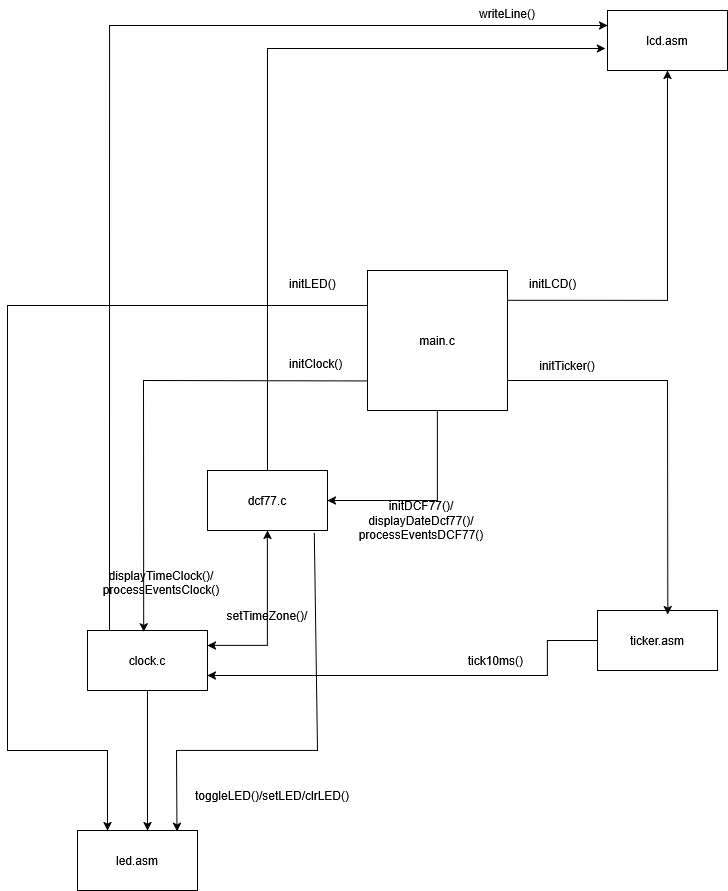
\includegraphics[width=1\textwidth]{diagrams/1.ModuleOverview.png}
    \caption{Module Overview}
    \label{fig:ModuleOverview}
\end{figure}

\newpage

% ---------------------------------------
% 6. Interface Descriptions of All Subroutines
% ---------------------------------------

\section{Interface Descriptions of All Subroutines}

% ---------------------------------------
% 6.1 main.c
% ---------------------------------------

\subsection{main.c}
\begin{itemize}
    \item \textbf{main()}  
    Initializes all modules and calls the corresponding subroutines.
\end{itemize}

% ---------------------------------------
% 6.2 clock.c
% ---------------------------------------

\subsection{clock.c}
\begin{itemize}
    \item \textbf{initClock()}  
    Loads the initial time and weekday.

    \item \textbf{tick10ms()}  
    Called every 10\,ms to advance internal clock logic.

    \item \textbf{processEventsClock(clockEvent)}  
    Updates internal time based on received event.

    \item \textbf{setClock(hours, minutes, seconds)}  
    Sets the current time, e.g. based on DCF77 data.

    \item \textbf{tzName()}  
    Returns the time zone abbreviation.

    \item \textbf{tzHours()}  
    Returns the time zone offset.

    \item \textbf{displayTimeClock()}  
    Writes current time to the LCD using \texttt{writeLine()}.

    \item \textbf{time()}  
    Returns the system uptime in milliseconds.
\end{itemize}

% ---------------------------------------
% 6.3 dcf77.c
% ---------------------------------------

\subsection{dcf77.c}
\begin{itemize}
    \item \textbf{initDCF77()}  
    Initializes the DCF77 module and decoder state.

    \item \textbf{initializePort()}  
    Configures Port H.0 for input signal polling.

    \item \textbf{readPort()}  
    Reads the DCF77 signal from Port H.0 (0 = LOW, 1 = HIGH).

    \item \textbf{sampleSignalDCF77(currentTime)}  
    Called every 10\,ms. Measures pulse durations and returns DCF77 events.

    \item \textbf{processEventsDCF77(event)}  
    Processes signal states via a DCF77 event state machine.

    \item \textbf{updateDate()}  
    Updates system date and time, and refreshes the display.

    \item \textbf{displayDateDcf77()}  
    Displays the decoded date on the LCD using \texttt{writeLine()}.

    \item \textbf{setDateDcf77()}  
    Validates the received data and updates internal variables.

    \item \textbf{verifyValue(start, end)}  
    Verifies a BCD-coded value including parity check.

    \item \textbf{setTimeZone(timeZone, hours, minutes)}  
    Sets the system time zone and applies the offset.
\end{itemize}

% ---------------------------------------
% 6.4 lcd.asm
% ---------------------------------------

\subsection{lcd.asm}
\begin{itemize}
    \item \textbf{writeLine(line, text)}  
    Displays a text string on the specified LCD line.
\end{itemize}

% ---------------------------------------
% 6.5 led.asm
% ---------------------------------------

\subsection{led.asm}
\begin{itemize}
    \item \textbf{initLED()}  
    Initializes the LED output pins on Port B.

    \item \textbf{setLED0(on)}  
    Toggles LED on Port B.0 every second.

    \item \textbf{setLED1(signal)}  
    Reflects raw DCF77 signal on Port B.1.

    \item \textbf{setLED2(error)}  
    Lights up Port B.2 if invalid data is detected.

    \item \textbf{setLED3(valid)}  
    Turns on Port B.3 when a valid DCF77 frame is decoded.
\end{itemize}

% ---------------------------------------
% 6.6 button.asm
% ---------------------------------------

\subsection{button.asm}
\begin{itemize}
    \item \textbf{USDE\_Pressed()}  
    Detects button press on PTH3 to toggle between DE and US time zones.
\end{itemize}

\newpage

% ---------------------------------------
% 7. Flow Charts
% ---------------------------------------

\section{Flow Charts}

% ---------------------------------------
% 7.1 Main
% ---------------------------------------

\subsection{Main}

\begin{figure}[H]
    \centering
    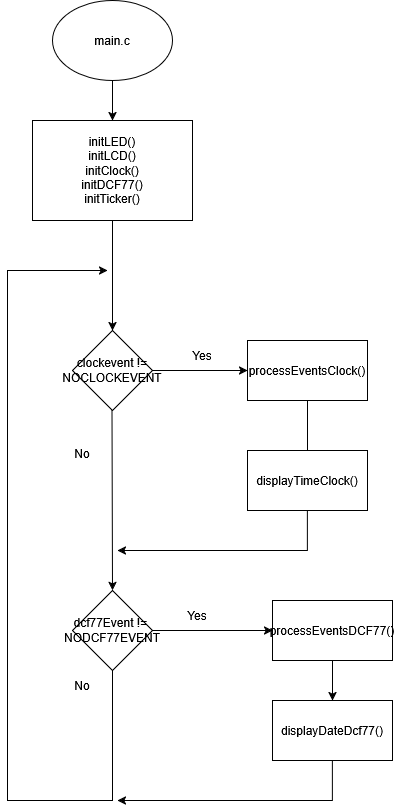
\includegraphics[width=0.6\textwidth]{diagrams/2.Main.png}
    \caption{Main}
    \label{fig:Main}
\end{figure}

% ---------------------------------------
% 7.2 Clock
% ---------------------------------------

\subsection{Clock}

\begin{figure}[H]
    \centering
    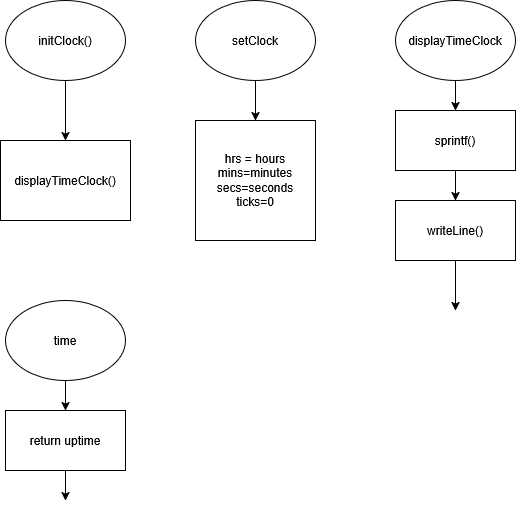
\includegraphics[width=1\textwidth]{diagrams/3.clock1.png}
    \caption{Clock 1}
    \label{fig:Clock1}
\end{figure}

\begin{figure}[H]
    \centering
    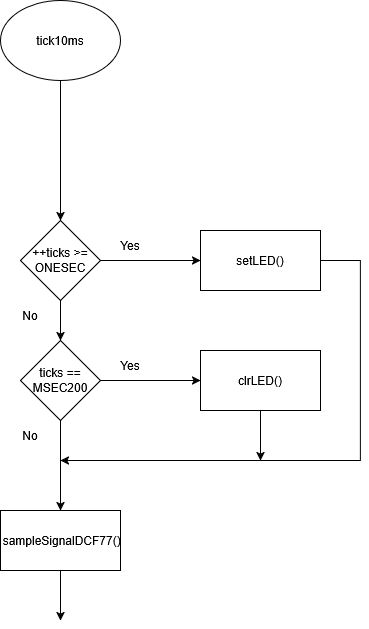
\includegraphics[width=0.8\textwidth]{diagrams/4.clock2.png}
    \caption{Clock 2}
    \label{fig:Clock2}
\end{figure}

% ---------------------------------------
% 7.3 DCF77
% ---------------------------------------

\subsection{DCF77}

\begin{figure}[H]
    \centering
    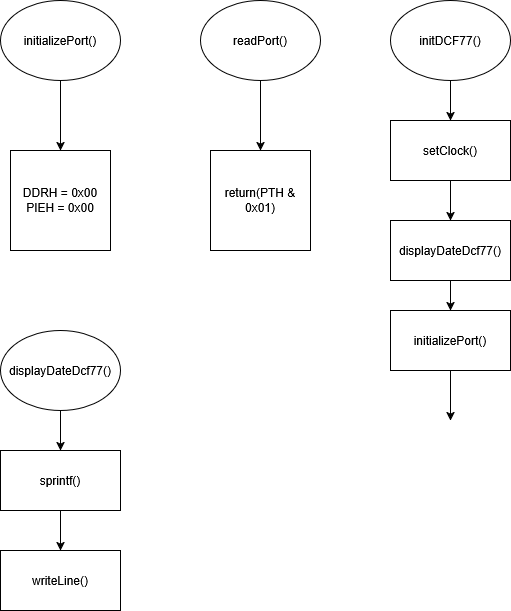
\includegraphics[width=0.8\textwidth]{diagrams/5.dcf771.png}
    \caption{DCF77 - Part 1}
    \label{fig:DCF77}
\end{figure}

\begin{figure}[H]
    \centering
    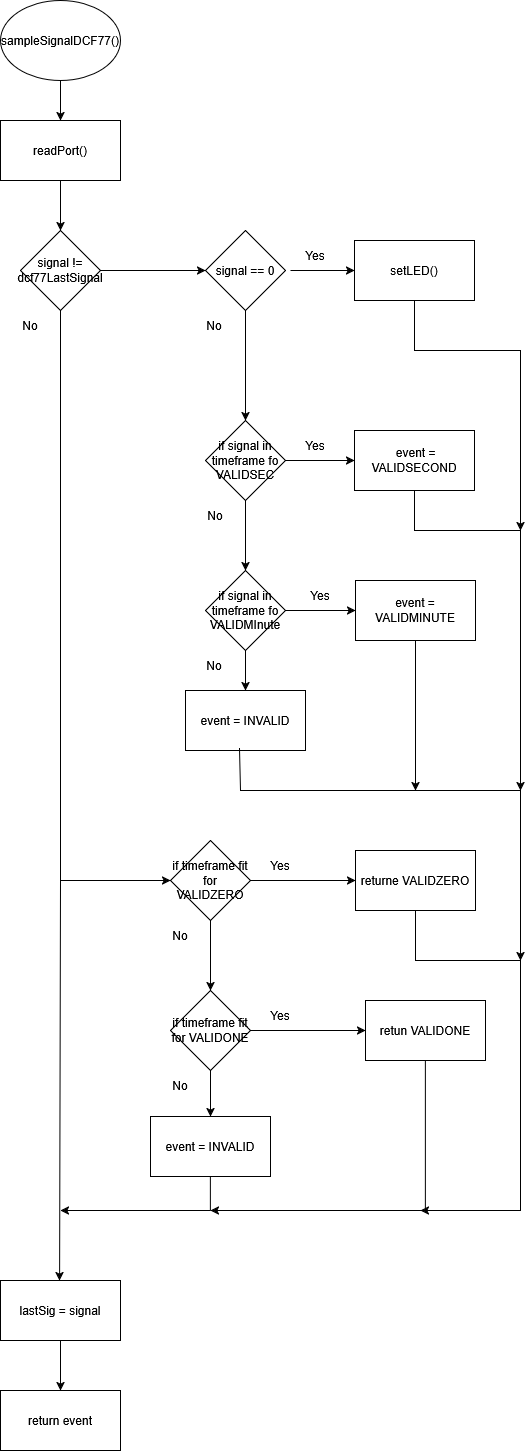
\includegraphics[width=0.525\textwidth]{diagrams/6.dcf772.png}
    \caption{DCF77 - Part 2}
    \label{fig:DCF772}
\end{figure}

\begin{figure}[H]
    \centering
    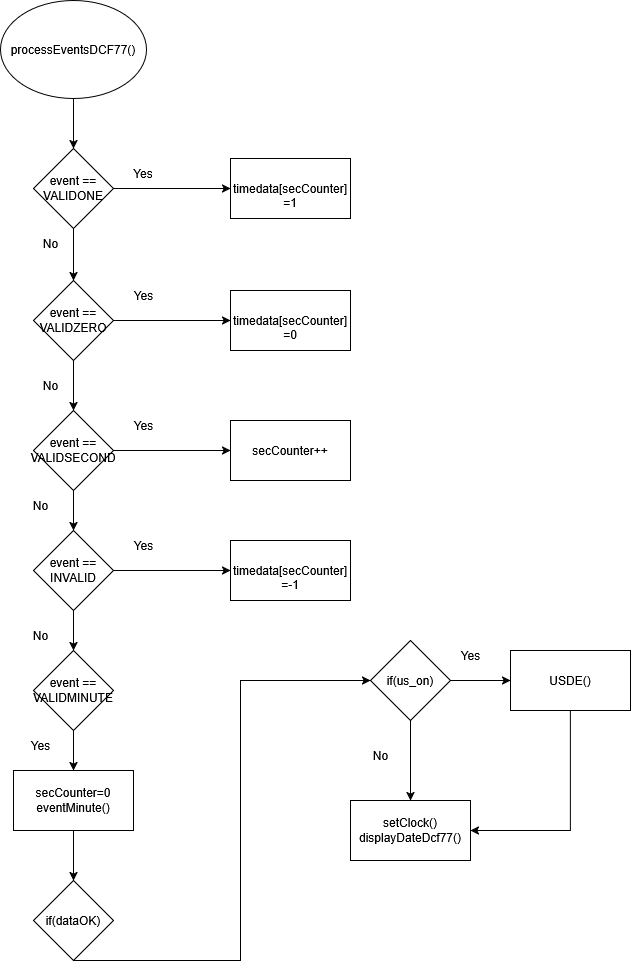
\includegraphics[width=0.95\textwidth]{diagrams/7.dcf773.png}
    \caption{DCF77 - Part 3}
    \label{fig:DCF773}
\end{figure}

\begin{figure}[H]
    \centering
    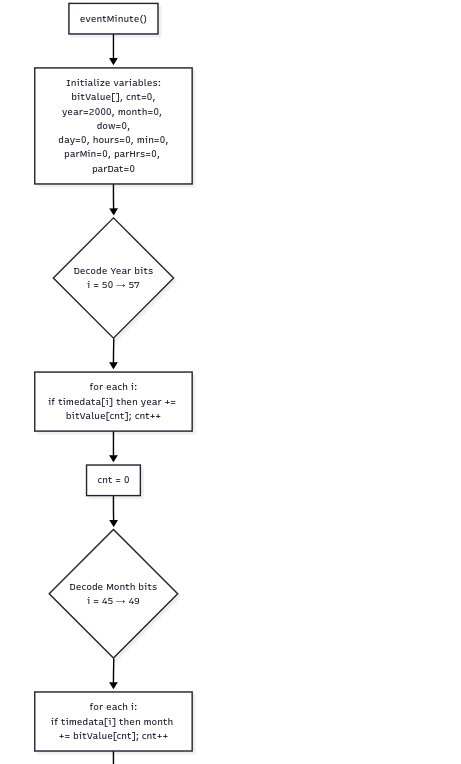
\includegraphics[width=0.7\textwidth]{diagrams/eventMinute/eventMinute1.png}
    \caption{Event Minute – Part 1}
    \label{fig:eventMinute1}
\end{figure}

\begin{figure}[H]
    \centering
    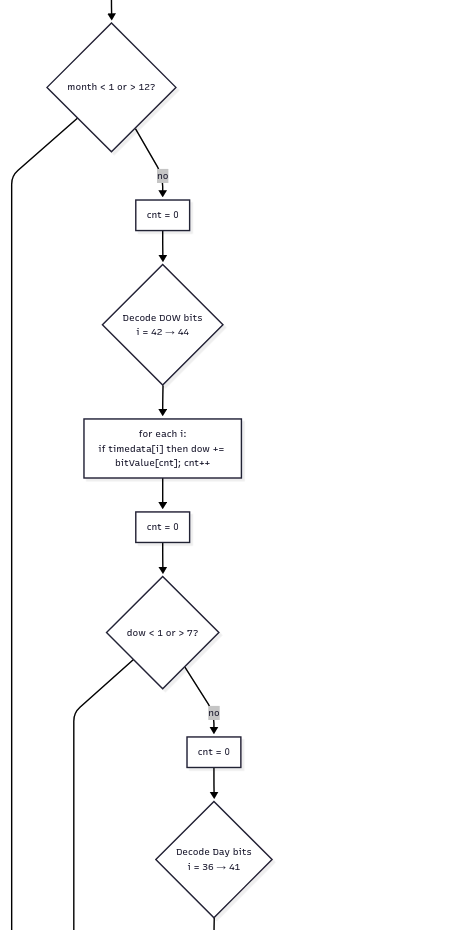
\includegraphics[width=0.7\textwidth]{diagrams/eventMinute/eventMinute2.png}
    \caption{Event Minute – Part 2}
    \label{fig:eventMinute2}
\end{figure}

\begin{figure}[H]
    \centering
    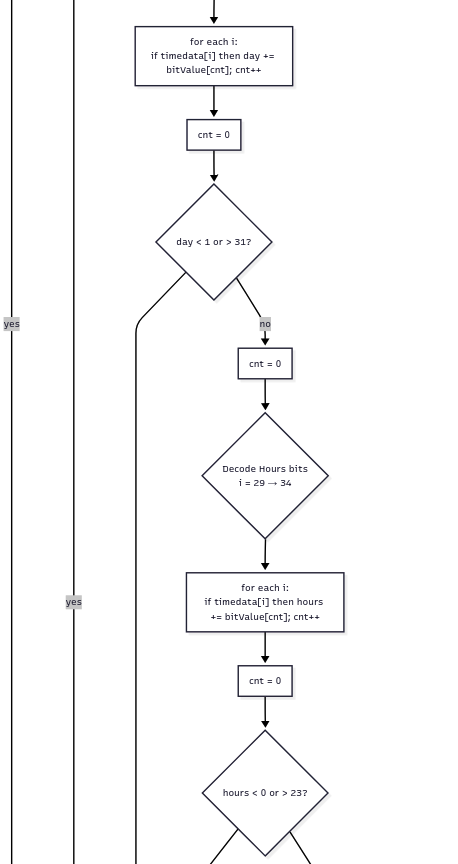
\includegraphics[width=0.7\textwidth]{diagrams/eventMinute/eventMinute3.png}
    \caption{Event Minute – Part 3}
    \label{fig:eventMinute3}
\end{figure}

\begin{figure}[H]
    \centering
    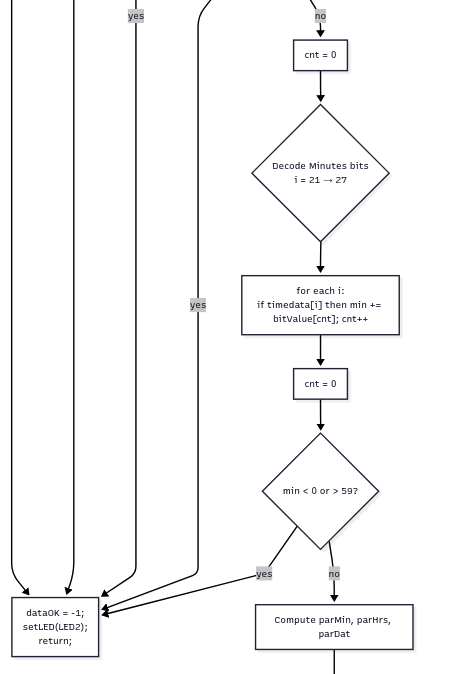
\includegraphics[width=0.7\textwidth]{diagrams/eventMinute/eventMinute4.png}
    \caption{Event Minute – Part 4}
    \label{fig:eventMinute4}
\end{figure}

\begin{figure}[H]
    \centering
    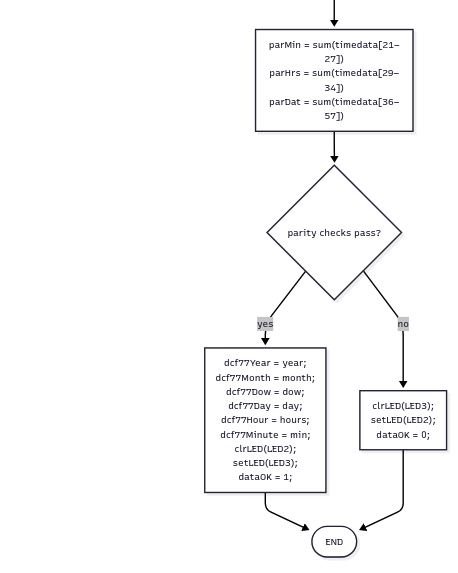
\includegraphics[width=0.7\textwidth]{diagrams/eventMinute/eventMinute5.png}
    \caption{Event Minute – Part 5}
    \label{fig:eventMinute5}
\end{figure}

\begin{figure}[H]
    \centering
    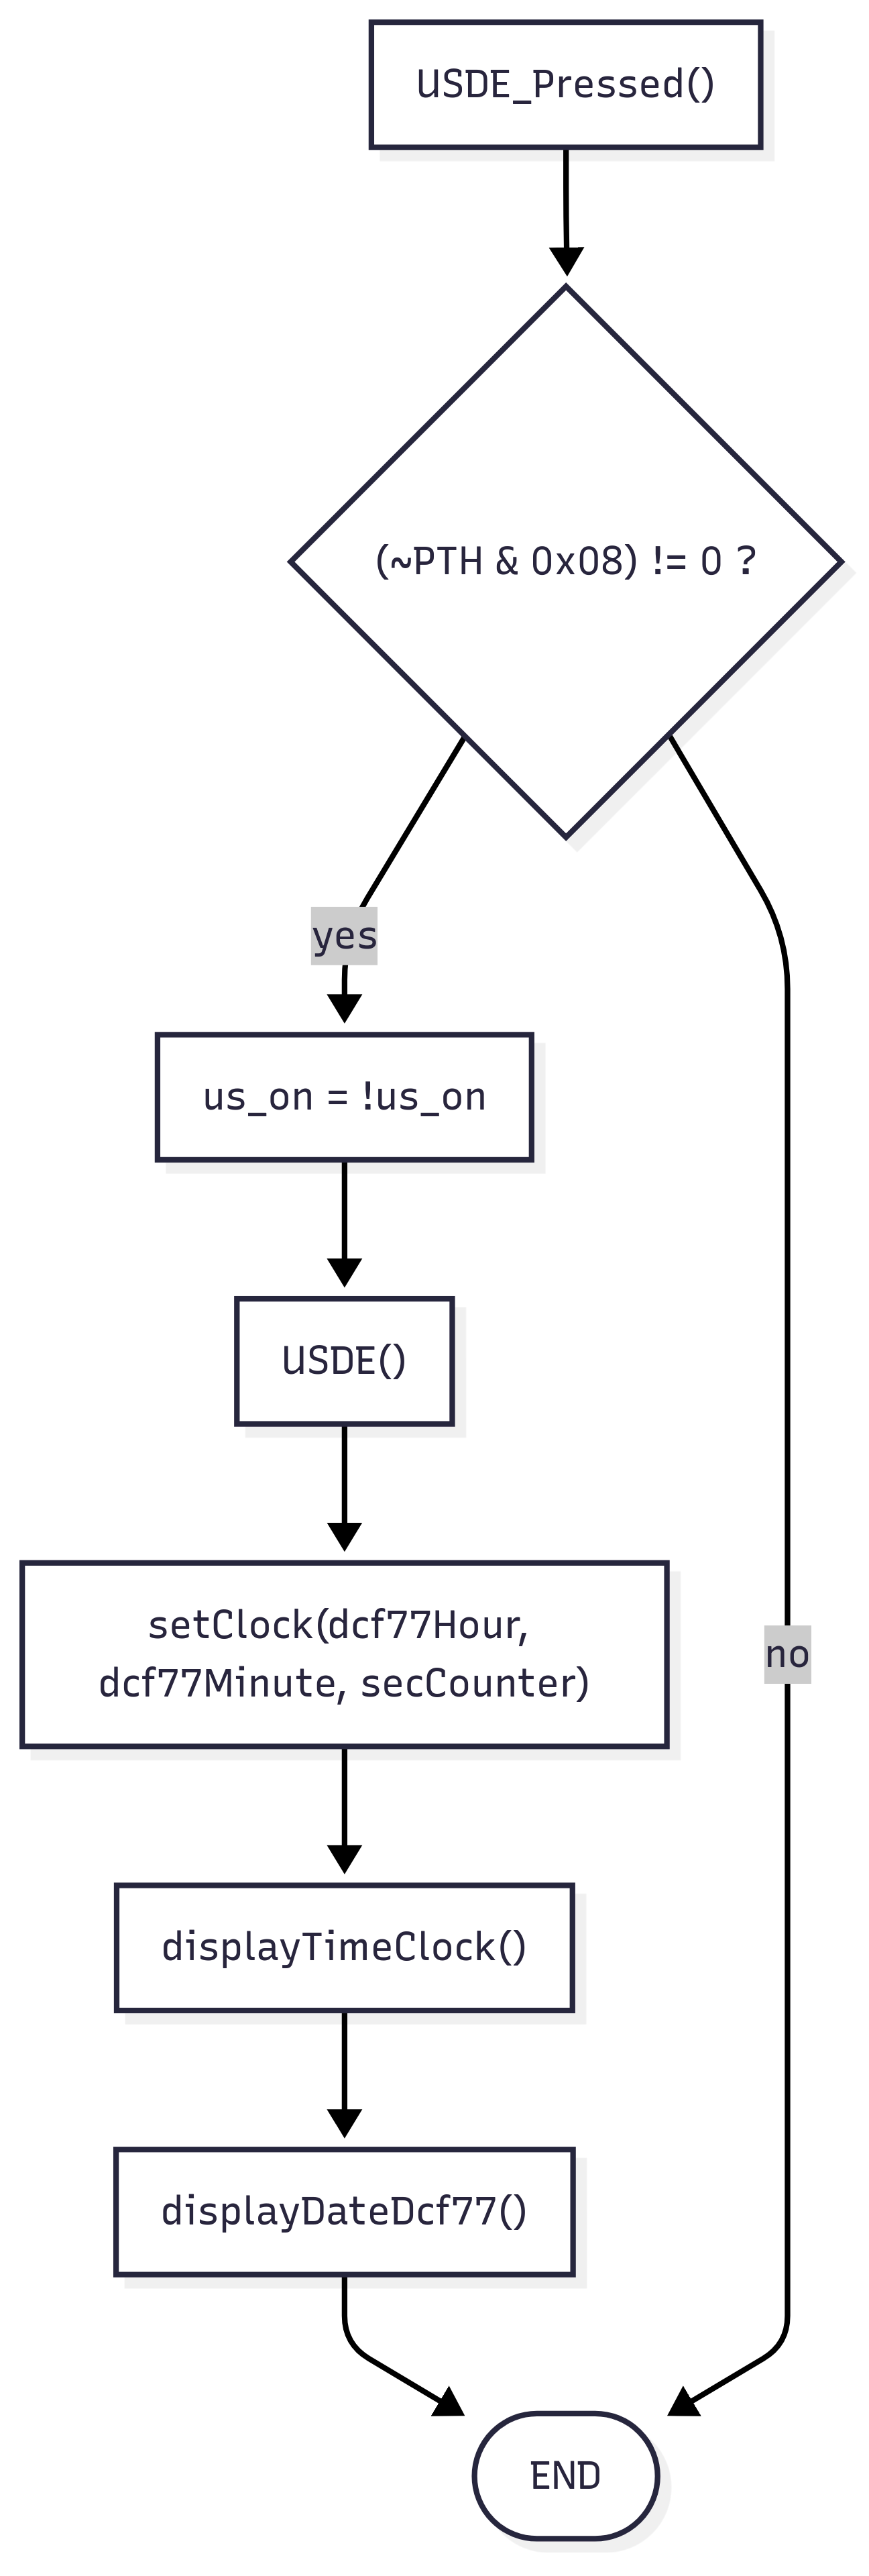
\includegraphics[width=0.45\textwidth]{diagrams/9.USDE_Pressed.png}
    \caption{USDE Pressed}
    \label{fig:USDEPressed}
\end{figure}

\begin{figure}[H]
    \centering
    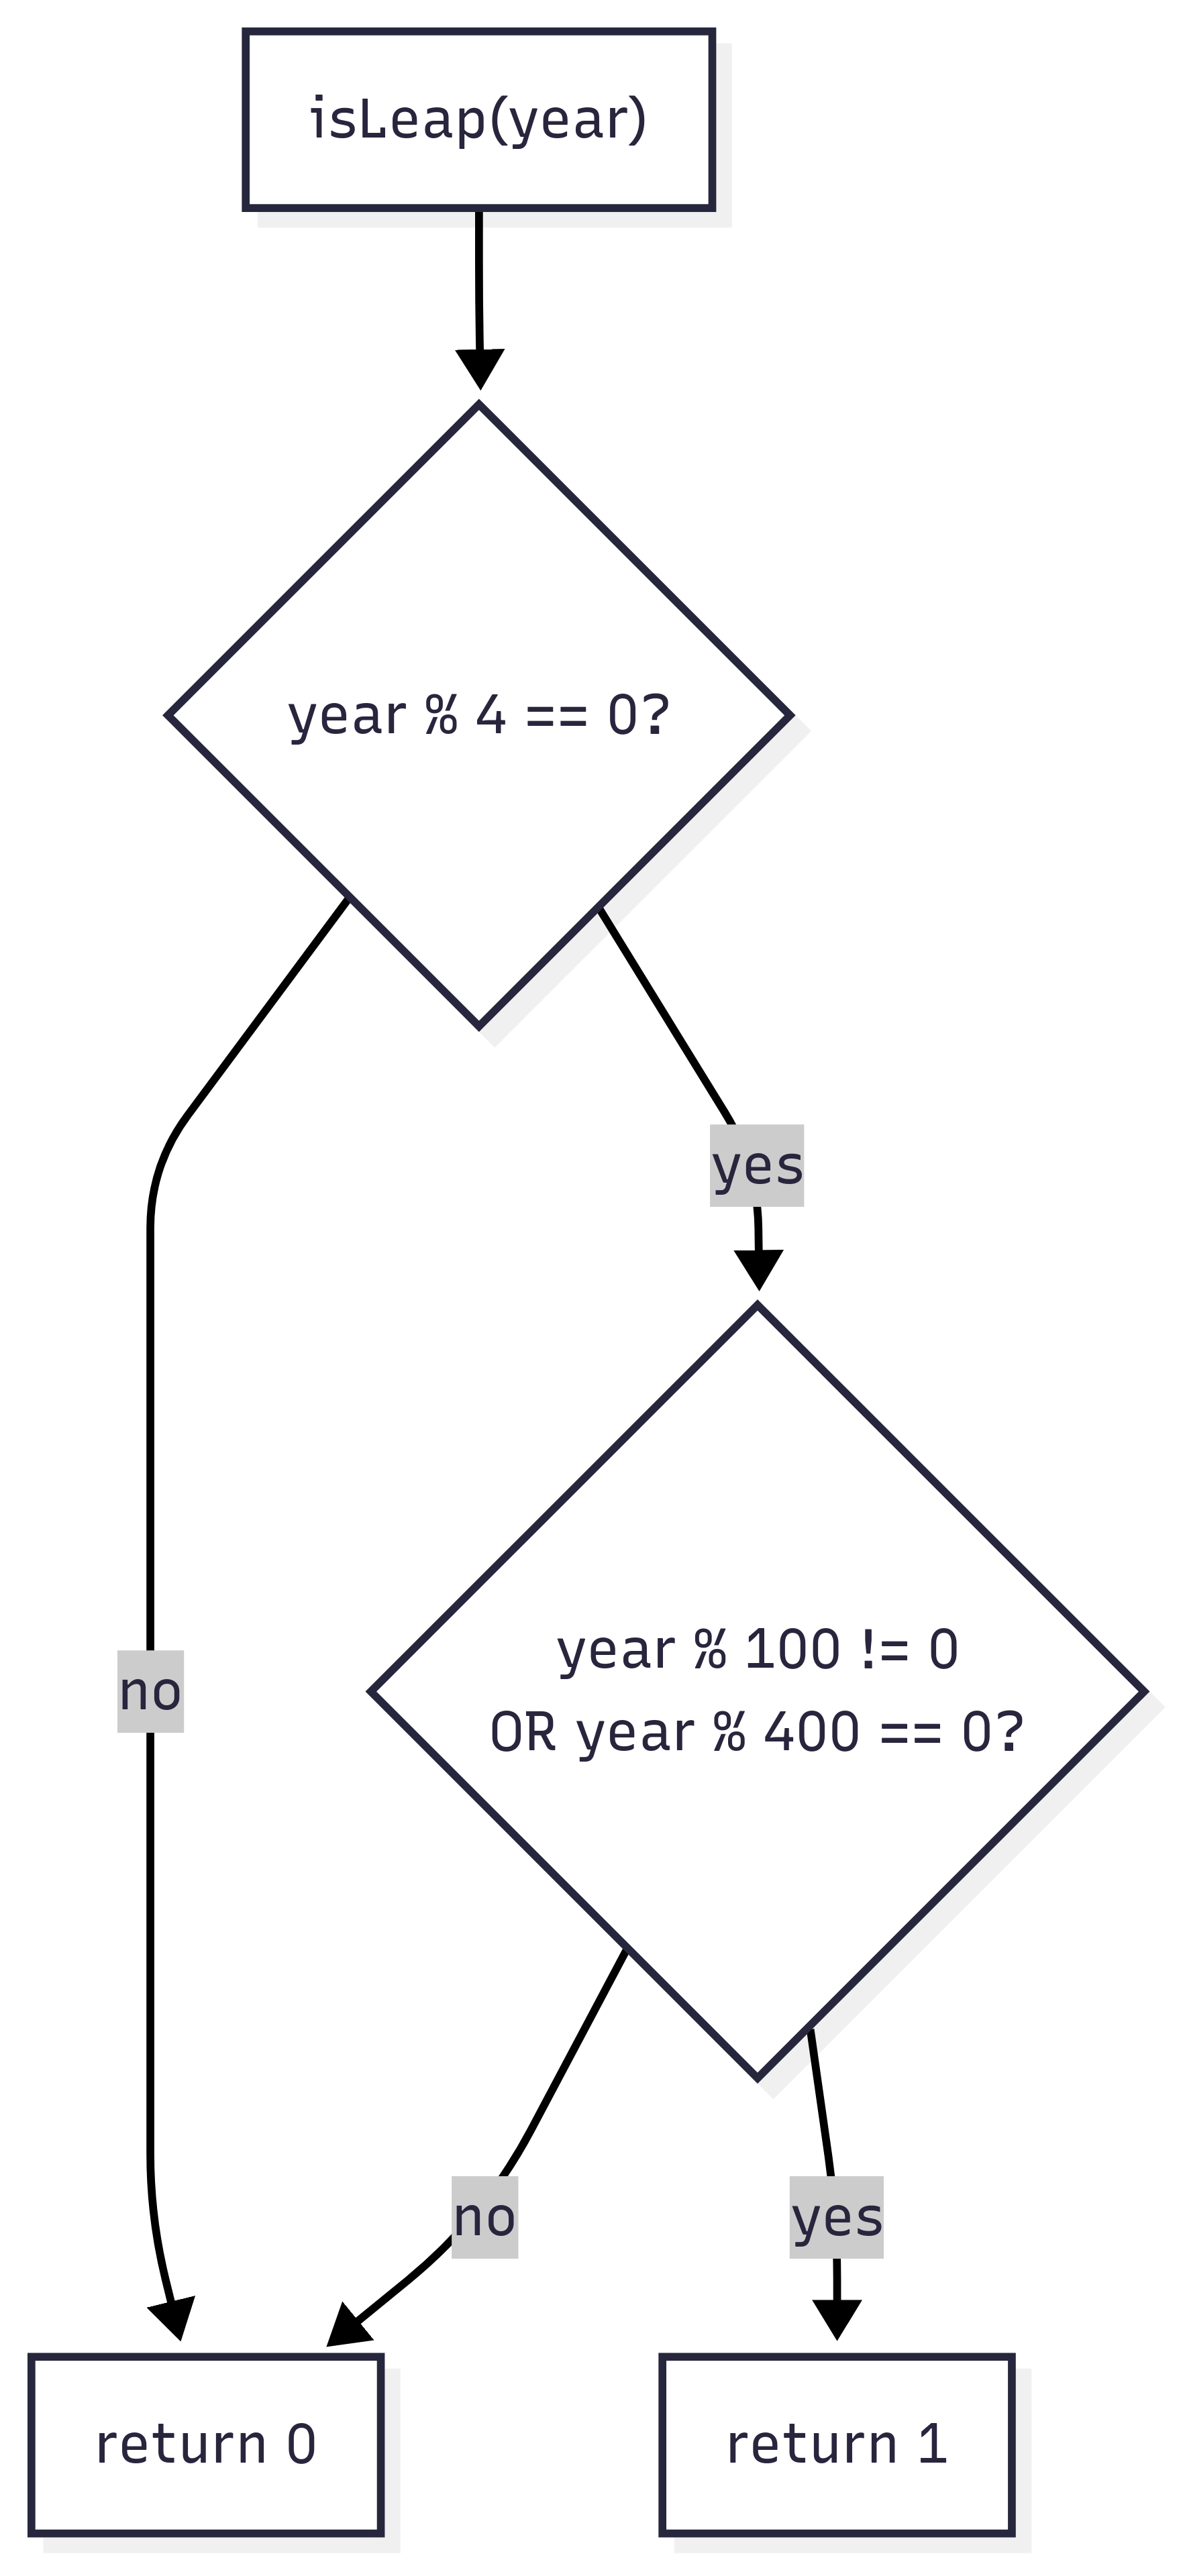
\includegraphics[width=0.5\textwidth]{diagrams/10.isLeap.png}
    \caption{isLeap}
    \label{fig:isLeap}
\end{figure}

\begin{figure}[H]
    \centering
    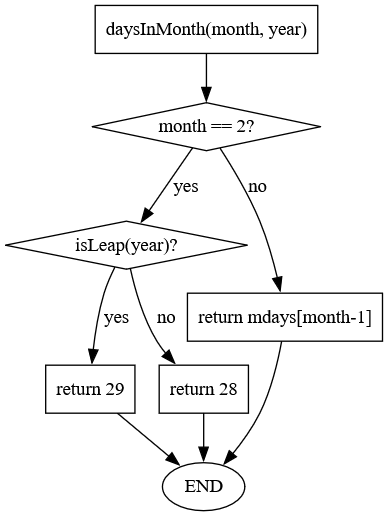
\includegraphics[width=0.7\textwidth]{diagrams/11.daysInMonth.png}
    \caption{daysInMonth}
    \label{fig:daysInMonth}
\end{figure}

\begin{figure}[H]
    \centering
    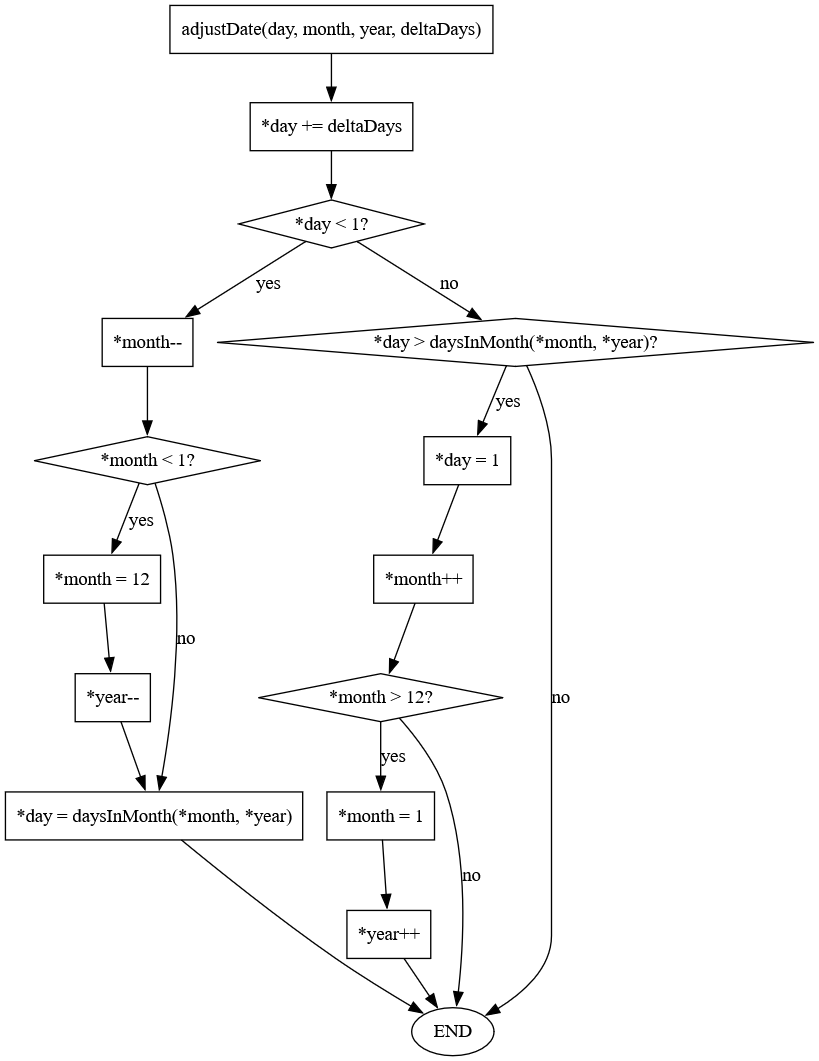
\includegraphics[width=0.9\textwidth]{diagrams/12.adjustDate.png}
    \caption{adjustDate}
    \label{fig:adjustDate}
\end{figure}

\begin{figure}[H]
    \centering
    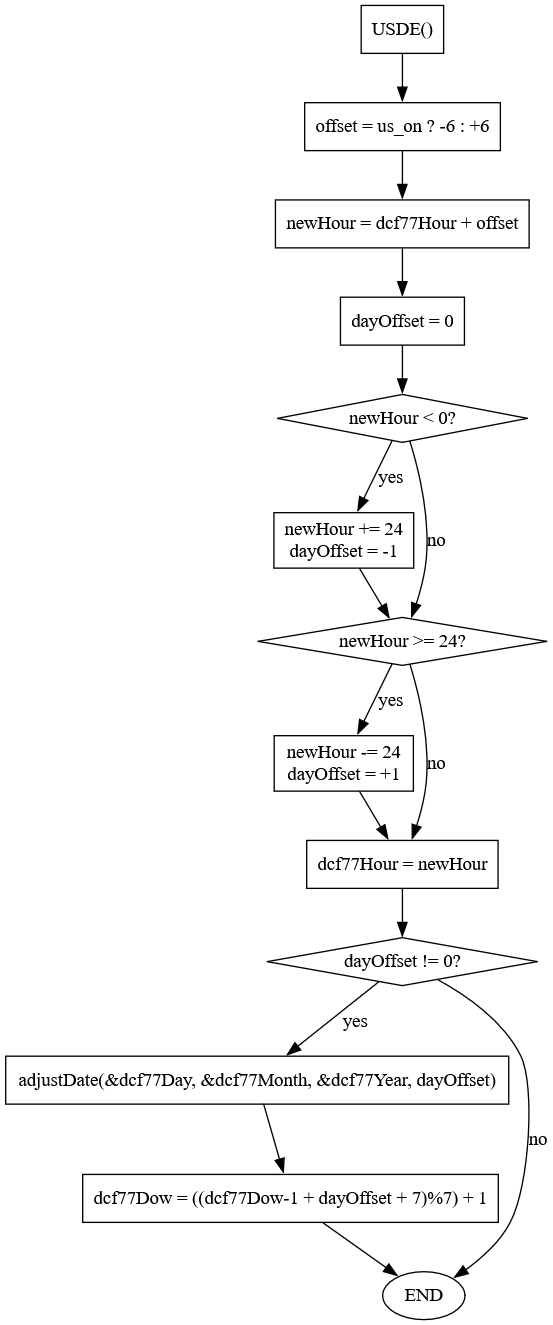
\includegraphics[width=0.55\textwidth]{diagrams/13.USDE.png}
    \caption{USDE}
    \label{fig:USDE}
\end{figure}

\end{document}
